\documentclass[a4paper,12pt]{article}
\usepackage[left=2.5cm, right=2.5cm, top=2cm, bottom=2cm]{geometry}

\usepackage[style=authoryear, maxcitenames=2, maxbibnames=3]{biblatex}
\addbibresource{ref.bib}

\usepackage{amsmath, amsfonts, amssymb, mathrsfs}
\usepackage{bm}
\usepackage{graphicx}
\usepackage{subcaption}
\usepackage{float}
\usepackage{hyperref}
\usepackage[labelsep=none]{caption}
\usepackage{textcomp}
\usepackage[T1]{fontenc}
\usepackage{booktabs}

\newcommand\independent{\protect\mathpalette{\protect\independenT}{\perp}}
\def\independenT#1#2{\mathrel{\rlap{$#1#2$}\mkern2mu{#1#2}}}

\DeclareMathAlphabet{\mathsfbr}{OT1}{cmss}{m}{n}%for math sans serif (cmss)
\SetMathAlphabet{\mathsfbr}{bold}{OT1}{cmss}{bx}{n}%for math sans serif (cmss)
\DeclareRobustCommand{\msf}[1]{%
  \ifcat\noexpand#1\relax\msfgreek{#1}\else\mathsfbr{#1}\fi%for math sans serif (cmss)
}

\DeclareRobustCommand{\mcal}[1]{%
  \ifcat\noexpand#1\relax\mathnormal{#1}\else\cal{#1}\fi
}
\DeclareRobustCommand{\BM}[1]{%
  \ifcat\noexpand#1\relax\bm{\boldUppercaseItalicGreek{#1}}\else\bm{#1}\fi
}

\makeatletter
\newcommand{\msfgreek}[1]{\csname s\expandafter\@gobble\string#1\endcsname}
\newcommand{\boldUppercaseItalicGreek}[1]{\csname var\expandafter\@gobble\string#1\endcsname}
\makeatother

%% Sans Serif Greek
\DeclareFontEncoding{LGR}{}{} % or load \usepackage{textgreek}
\DeclareSymbolFont{sfgreek}{LGR}{cmss}{m}{n}
\SetSymbolFont{sfgreek}{bold}{LGR}{cmss}{bx}{n}
\DeclareMathSymbol{\salpha}{\mathord}{sfgreek}{`a}
\DeclareMathSymbol{\sbeta}{\mathord}{sfgreek}{`b}
\DeclareMathSymbol{\sgamma}{\mathord}{sfgreek}{`g}
\DeclareMathSymbol{\sdelta}{\mathord}{sfgreek}{`d}
\DeclareMathSymbol{\sepsilon}{\mathord}{sfgreek}{`e}
\DeclareMathSymbol{\szeta}{\mathord}{sfgreek}{`z}
\DeclareMathSymbol{\seta}{\mathord}{sfgreek}{`h}
\DeclareMathSymbol{\stheta}{\mathord}{sfgreek}{`j}
\DeclareMathSymbol{\siota}{\mathord}{sfgreek}{`i}
\DeclareMathSymbol{\skappa}{\mathord}{sfgreek}{`k}
\DeclareMathSymbol{\slambda}{\mathord}{sfgreek}{`l}
\DeclareMathSymbol{\smu}{\mathord}{sfgreek}{`m}
\DeclareMathSymbol{\snu}{\mathord}{sfgreek}{`n}
\DeclareMathSymbol{\sxi}{\mathord}{sfgreek}{`x}
\DeclareMathSymbol{\somicron}{\mathord}{sfgreek}{`o}
\DeclareMathSymbol{\spi}{\mathord}{sfgreek}{`p}
\DeclareMathSymbol{\srho}{\mathord}{sfgreek}{`r}
\DeclareMathSymbol{\ssigma}{\mathord}{sfgreek}{`s}
\DeclareMathSymbol{\stau}{\mathord}{sfgreek}{`t}
\DeclareMathSymbol{\supsilon}{\mathord}{sfgreek}{`u}
\DeclareMathSymbol{\sphi}{\mathord}{sfgreek}{`f}
\DeclareMathSymbol{\schi}{\mathord}{sfgreek}{`q}
\DeclareMathSymbol{\spsi}{\mathord}{sfgreek}{`y}
\DeclareMathSymbol{\somega}{\mathord}{sfgreek}{`w}
\let\svarepsilon\sepsilon
\let\svartheta\stheta
\let\svarpi\spi
\let\svarrho\srho
\DeclareMathSymbol{\svarsigma}{\mathord}{sfgreek}{`c}
\let\svarphi\sphi
\DeclareMathSymbol{\sGamma}{\mathalpha}{sfgreek}{`G}
\DeclareMathSymbol{\sDelta}{\mathalpha}{sfgreek}{`D}
\DeclareMathSymbol{\sTheta}{\mathalpha}{sfgreek}{`J}
\DeclareMathSymbol{\sLambda}{\mathalpha}{sfgreek}{`L}
\DeclareMathSymbol{\sXi}{\mathalpha}{sfgreek}{`X}
\DeclareMathSymbol{\sPi}{\mathalpha}{sfgreek}{`P}
\DeclareMathSymbol{\sSigma}{\mathalpha}{sfgreek}{`S}
\DeclareMathSymbol{\sUpsilon}{\mathalpha}{sfgreek}{`U}
\DeclareMathSymbol{\sPhi}{\mathalpha}{sfgreek}{`F}
\DeclareMathSymbol{\sPsi}{\mathalpha}{sfgreek}{`Y}
\DeclareMathSymbol{\sOmega}{\mathalpha}{sfgreek}{`W}

%% Math symbol command
\newcommand{\V}[1]{\bm{#1}} %%  vector
\newcommand{\M}[1]{\BM{#1}} %%  matrix
\newcommand{\Set}[1]{\mcal{#1}} %%  set
\newcommand{\rv}[1]{\MakeLowercase{\msf{#1}}} %% random variable
\newcommand{\RV}[1]{\bm{\MakeLowercase{\msf{#1}}}}  %% random vector
\newcommand{\RM}[1]{\bm{\MakeUppercase{\msf{#1}}}}  %% random matrix
\newcommand{\RS}[1]{\MakeUppercase{\msf{#1}}} %% random set


\begin{document}

\begin{center}
    Natual Language Processsing\\
    Spring 2025\\
    \vspace{0.25cm}
	\underline{\textbf{Assignment 2}}\\
    \vspace{0.5cm}
    \textbf{Name} \ \underline{Ke Li}  \hfill \textbf{Student No.} \ \underline{2024210837} \\
    \vspace{0.1cm}
\end{center}
\hrule
\vspace{0.2cm}

\section{Prompt Engirneering}

\subsection{Designing a Unique and Challenging Prompt}
\subsubsection{Model Selection}

Because our purpose is to generate a task that only one model can perform correctly, while the other model cannot, we need to find differences between the two models. A simple aspect is the model size, the larger model remembers more knowledge. However, this may not be the best choice, as we do not know which data is used to train one model and not the other. So I choose to distinguish the two models by their reasoning ability. Since \textbf{Deepseek-R1}(which is just Deepseek-V3 with deep thinking) has a better reasoning ability than \textbf{GPT-4o}, which is the true in its technique report (\cite{deepseekai2025deepseekr1incentivizingreasoningcapability}), I decide to use these two models to generate the task.

\subsubsection{Task Generation}

The question should have a single objective and easily verifiable answer, so mathematical problems are a good choice. Deepseek-R1 has reported their results in different math problems, so I choose the dataset which has the biggest difference pass@1 score between the two models, \href{https://www.modelscope.cn/datasets/AI-ModelScope/AIME_2024/summary}{AIME 2024}. The question I choose is:
\begin{quote}
    \textbf{Q:} Alice and Bob play the following game. A stack of $n$ tokens lies before them. The players take turns with Alice going first. On each turn, the player removes either $1$ token or $4$ tokens from the stack. Whoever removes the last token wins. Find the number of positive integers $n$ less than or equal to $2024$ for which there exists a strategy for Bob that guarantees that Bob will win the game regardless of Alice's play.
\end{quote}

The question ID is \textbf{2024-I-3}, and the answer is \textbf{809}. During my test, I find that GPT-4o can generate the answer quickly, but the results are not correct. In three tests, the answers are \textbf{899}, \textbf{810}, and \textbf{810}. They are all wrong. However, Deepseek-R1 can generate the answer correctly in all three tests. The results are \textbf{809}, \textbf{809}, and \textbf{809}. Despite the correctness, the time cost of Deepseek-R1 is much higher than GPT-4o. The time cost of Deepseek-R1 is \textbf{198s}, \textbf{179s}, and \textbf{138s}. I find an interesting phenomenon that although Deepseek-R1 has gotten the correct answer, it will "wait" and try another method to verify the answer, which causes the time cost to be much higher than GPT-4o. 

\subsubsection{Results}

Screen shots of the results are shown in Figure \ref{fig:4o_images} and Figure \ref{fig:dsr1_images}. 

\begin{figure}[H]
    \begin{subfigure}[b]{\textwidth}
        \centering
        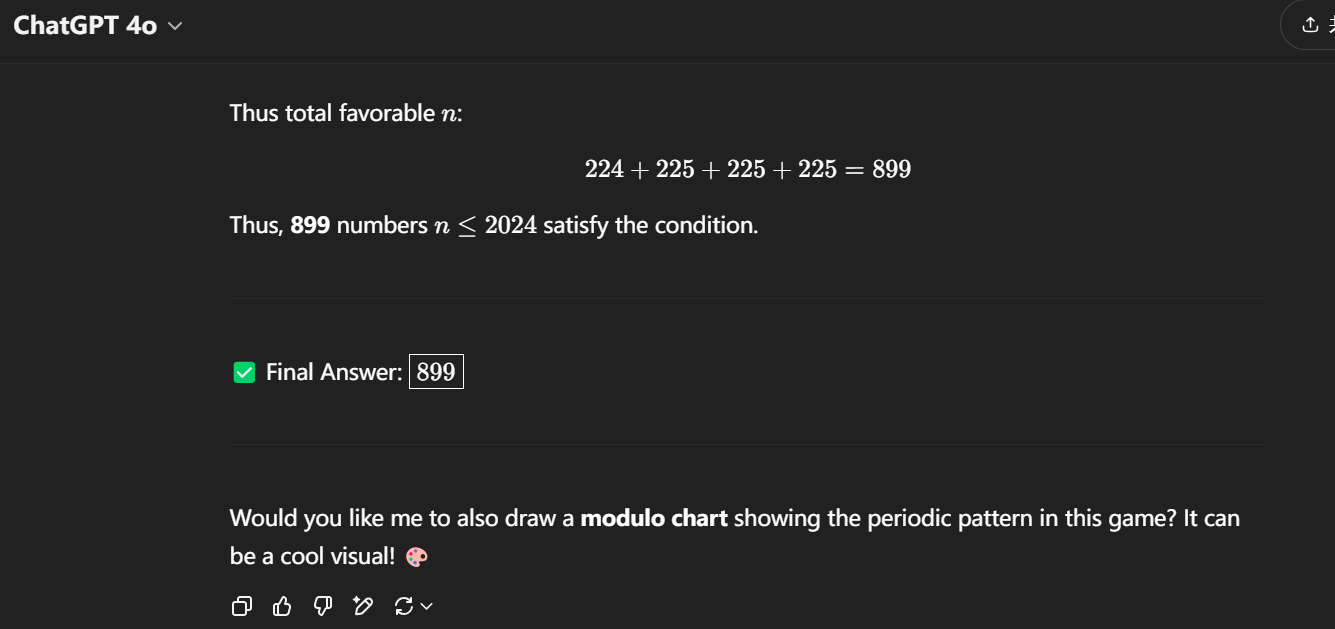
\includegraphics[width=0.8\textwidth]{figures/4o_1.png}
        \caption{GPT-4o result 1}
        \label{fig:image1}
    \end{subfigure}
    
    % 第二张图片
    \begin{subfigure}[b]{\textwidth}
        \centering
        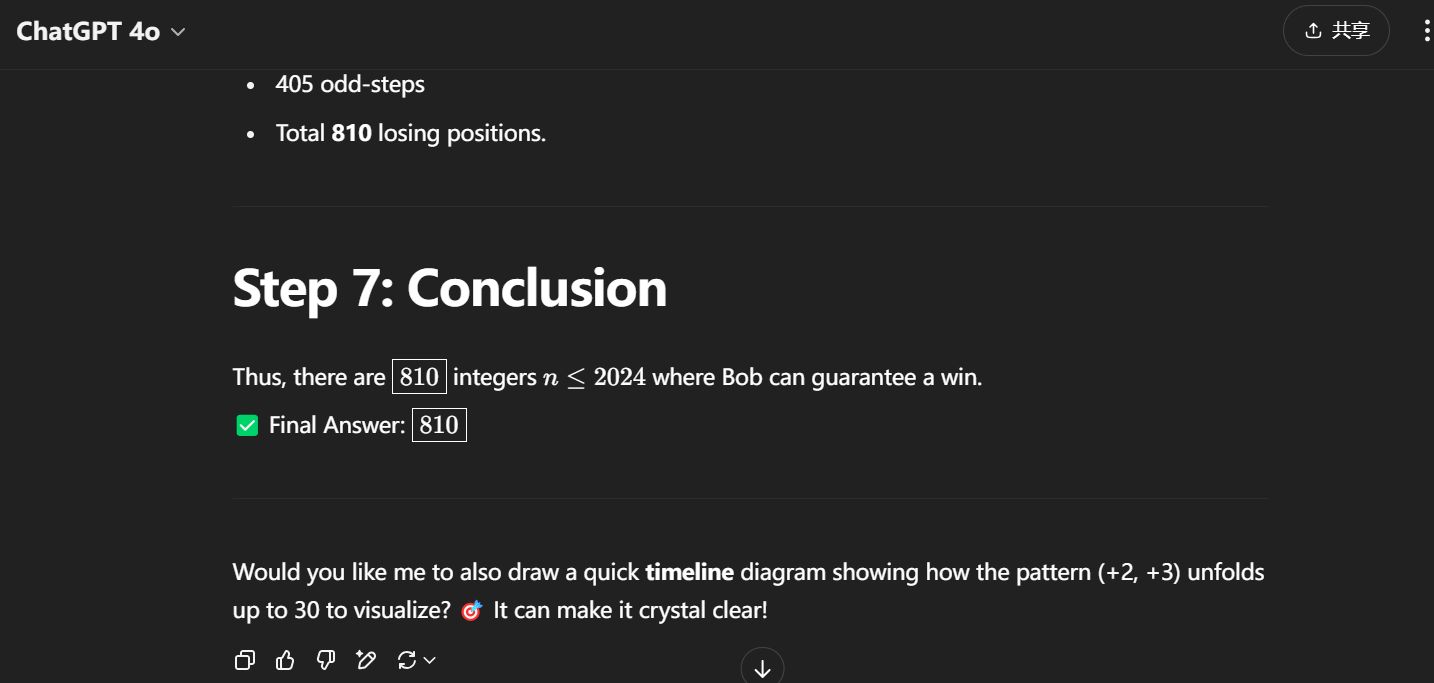
\includegraphics[width=0.8\textwidth]{figures/4o_2.png}
        \caption{GPT-4o result 2}
        \label{fig:image2}
    \end{subfigure}
    
    % 第三张图片
    \begin{subfigure}[b]{\textwidth}
        \centering
        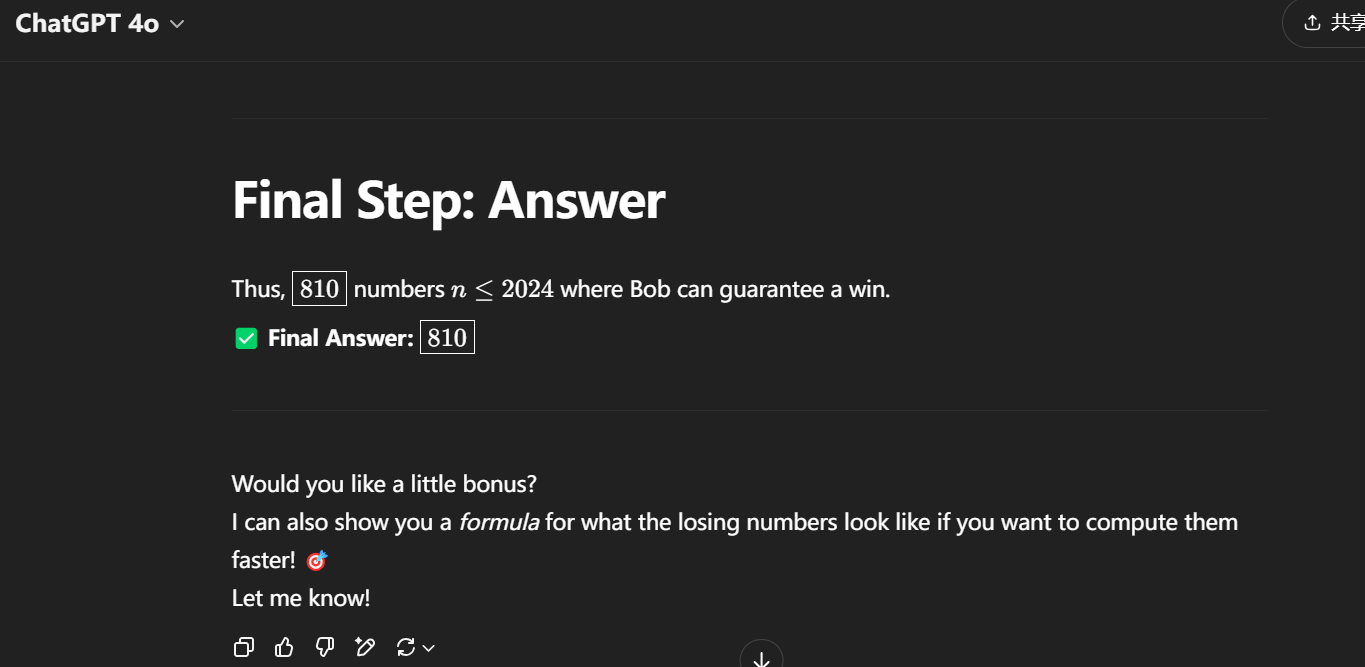
\includegraphics[width=0.8\textwidth]{figures/4o_3.png}
        \caption{GPT-4o result 3}
        \label{fig:image3}
    \end{subfigure}
    
    \caption{GPT-4o results}
    \label{fig:4o_images}
\end{figure}

\begin{figure}
    \begin{subfigure}[b]{\textwidth}
        \centering
        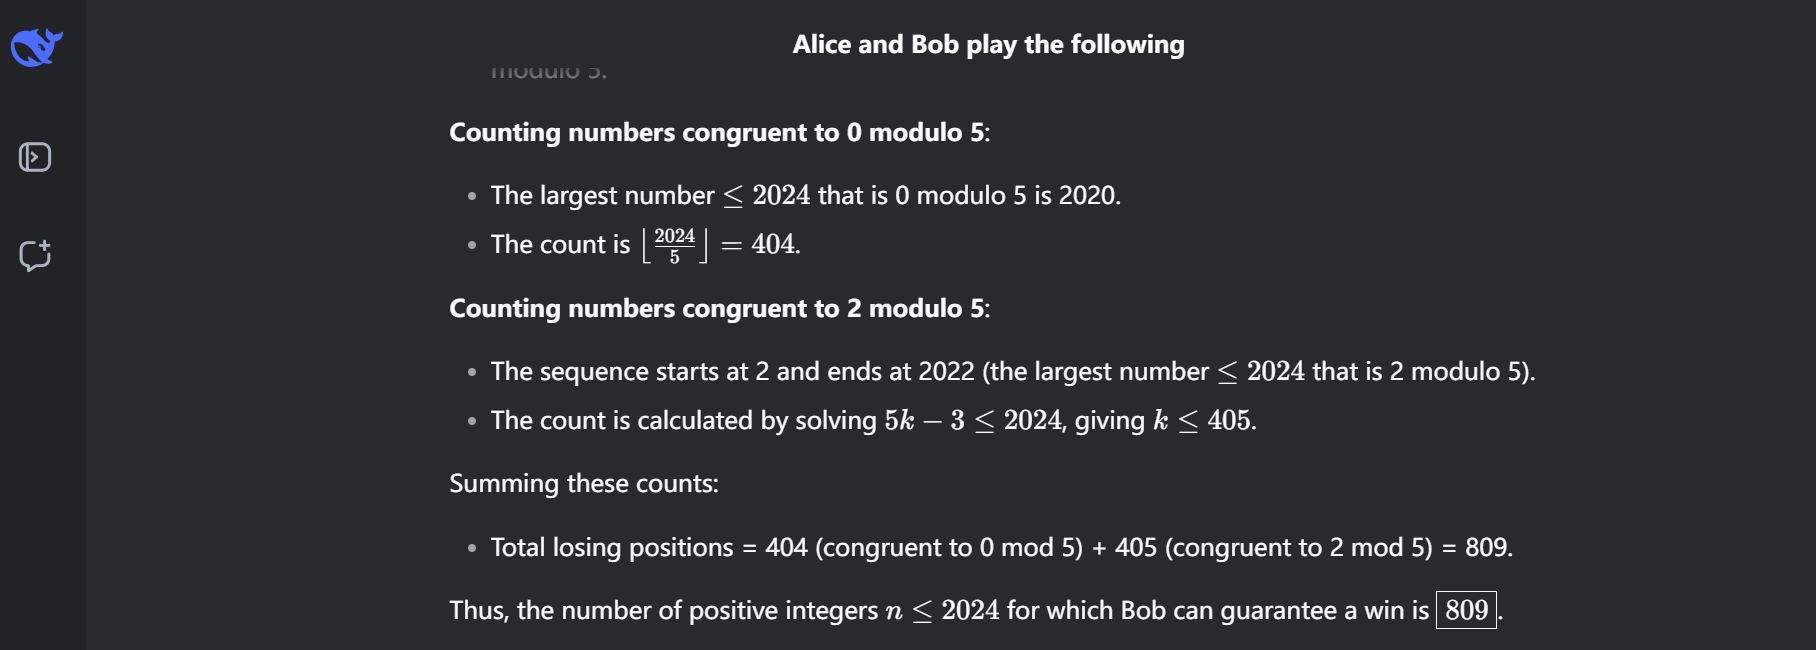
\includegraphics[width=0.8\textwidth]{figures/r1_198s.png}
        \caption{Deepseek-R1 result 1}
        \label{fig:image4}
    \end{subfigure}
    
  
    \begin{subfigure}[b]{\textwidth}
        \centering
        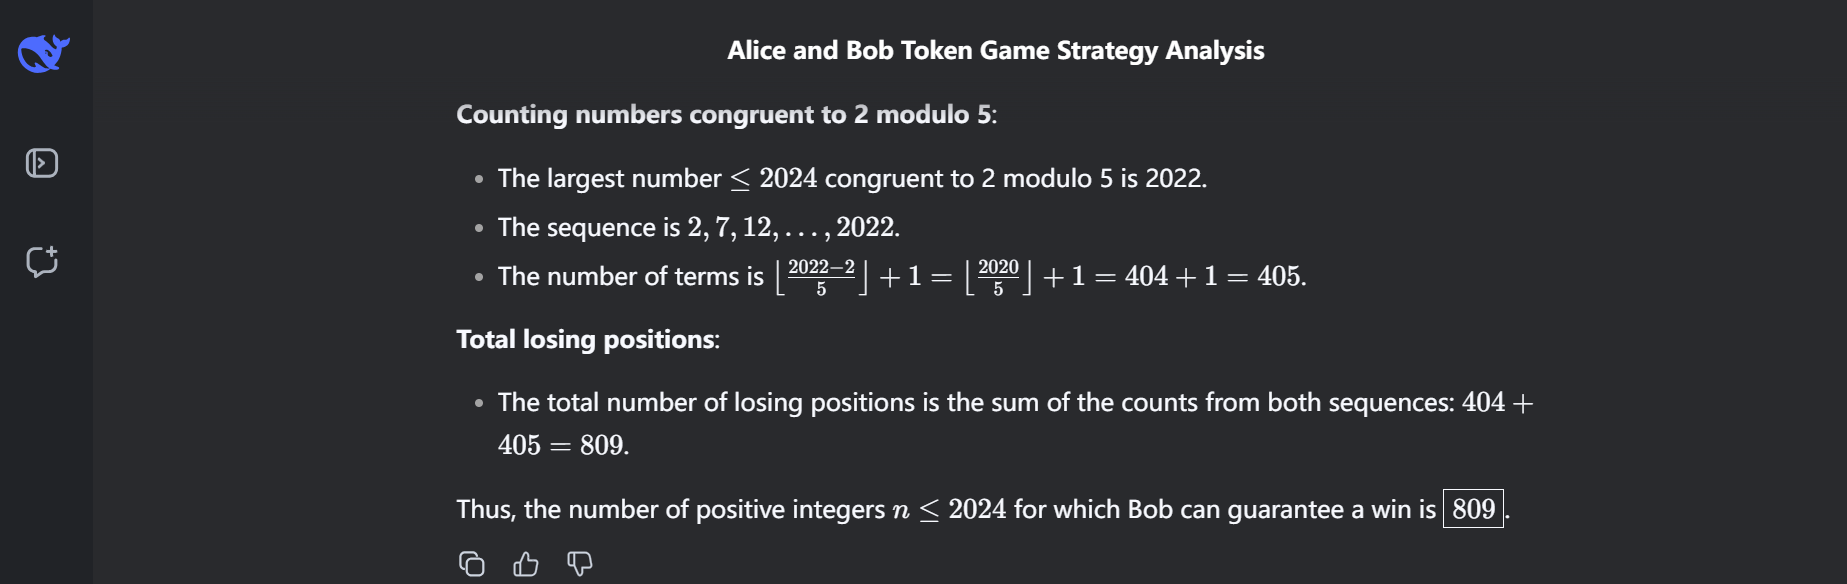
\includegraphics[width=0.8\textwidth]{figures/r1_179s.png}
        \caption{Deepseek-R1 result 2}
        \label{fig:image5}
    \end{subfigure}
    
    \begin{subfigure}[b]{\textwidth}
        \centering
        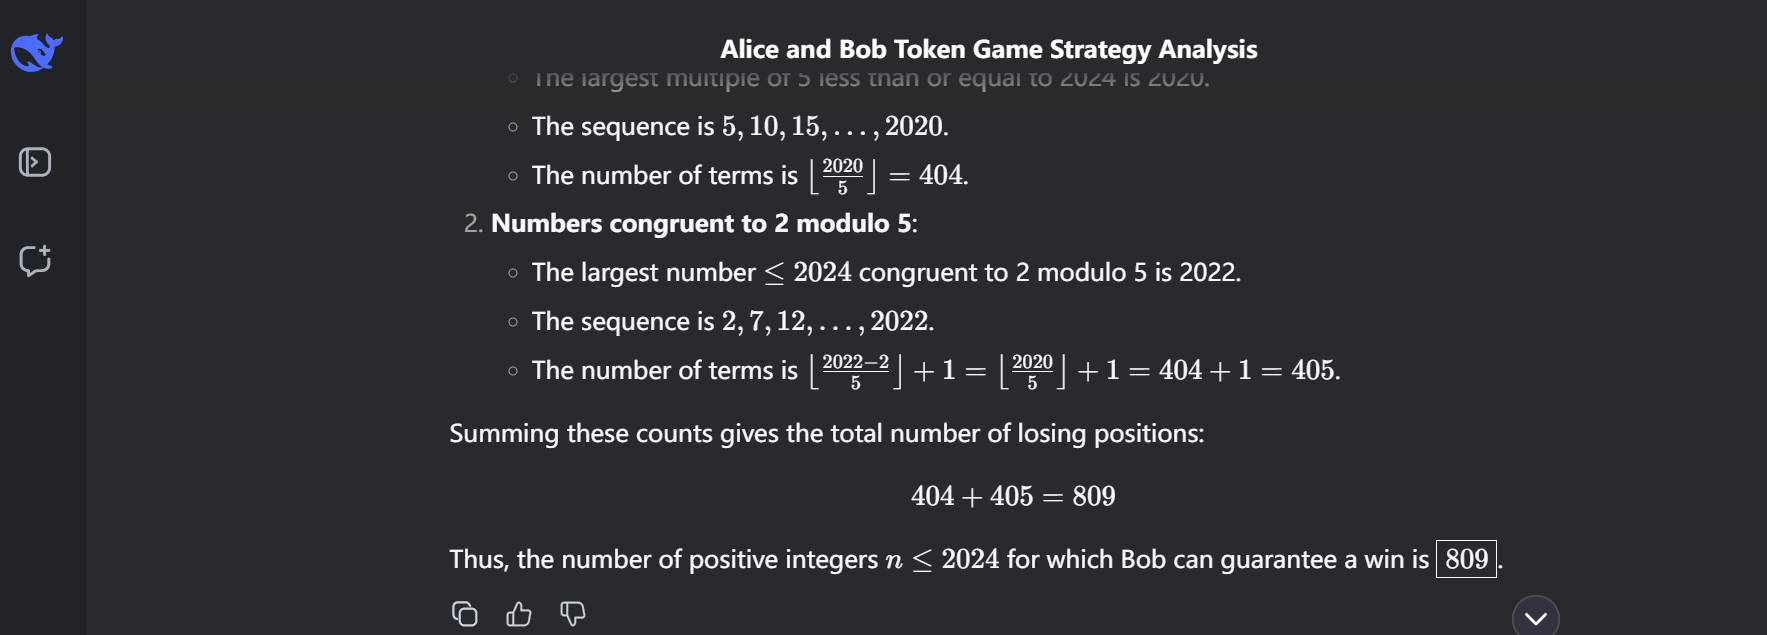
\includegraphics[width=0.8\textwidth]{figures/r1_138s.png}
        \caption{Deepseek-R1 result 3}
        \label{fig:image6}
    \end{subfigure}
    
    \caption{Deepseek-R1 results}
    \label{fig:dsr1_images}
\end{figure}


\printbibliography[heading=bibintoc, title={References}]

\end{document}
